\begin{figure*}[htb]
  \centering
  \begin{subfigure}[t]{0.33\textwidth}
    \centering
    \includegraphics[width=\textwidth]{figures/profile-mot.pdf}
    \caption{Pedestrian Detection}
    \label{fig:pd-profile}
  \end{subfigure}
  \hfill
  \begin{subfigure}[t]{0.33\textwidth}
    \centering
    \includegraphics[width=\textwidth]{figures/profile-darknet.pdf}
    \caption{Augmented Reality}
    \label{fig:ar-profile}
  \end{subfigure}
  \hfill
  \begin{subfigure}[t]{0.33\textwidth}
    \centering
    \includegraphics[width=\textwidth]{figures/profile-topk.pdf}
    \caption{Top-k}
    \label{fig:tk-profile}
  \end{subfigure}
  \caption{Application profiles.}
  \label{fig:all-profiles}
\end{figure*}

\section{Evaluation}
\label{sec:evaluation}

In this section, we show our evaluations of \sysname{}.

\begin{itemize}
\item[\autoref{sec:application-profiles}] \sysname{} is able to generate
  Pareto-optimal application profiles with precision and fine
  granularity. (\autoref{fig:all-profiles})
\item[\autoref{sec:online-profiling}] With our parallel profiling and selective
  triggering, \sysname{} keeps the adaptation model up to date with only 10\%
  GPU time. (\autoref{fig:parallel}, \autoref{fig:online-tricks})
\item[\autoref{sec:runtime-adaptation}] In comparison to applications built
  without adaptation suffer from large lag (TCP) or severe performance
  degradation (UDP), \sysname{} applications achieves bounded latency (1 seconds
  for video analytics and 5 seconds for log analysis) while incurring little
  accuracy loss. (\autoref{fig:all-runtime})
\item[\autoref{sec:multi-task-sched}] The profiles we learned for each
  application can also be used for allocating resources among multiple
  tasks. (\autoref{fig:multitask})
\end{itemize}

\subsection{Application Profiles}
\label{sec:application-profiles}

Our system learned the application profiles for all three applications (shown in
\autoref{fig:all-profiles}). From these profiles, we make the following three
observations:

\para{Optimal strategy is achieved with multiple dimensions.} In each profile,
in addition to the Pareto-optimal strategies, we show the performance if only
one dimension is tuned. As show in the figure, they almost always lead to a
sub-optimal performance.

\para{Different dimensions have different impact for the same application.}
For pedestrian detection, tuning resolution leads to a quicker degradation in
comparison to tuning frame rate.

\para{The same dimension has different impact for different applications.}
If we compare two video analytics applications, pedestrian detection and
augmented reality, we see how tuning each dimension affects the performance
differently.

\subsection{Efficient Online Profiling}
\label{sec:online-profiling}

First, we validate the necessity for online profiling. We compare two adaptation
scheme: one with the offline learned profile; the other enabled with online
profiling. Initially, both schemes work similarly. Overtime, when the data
distribution changes, the offline-learned profile doesn't match with the newly
generated data, leading to accuracy deterioration. System enabled with online
profiling is able to track the data and offers high accuracy.

While online profiling is beneficial, doing it naively faces the combinatorial
space search. This is different from the offline profiling that doesn't have
much time or resource constrain. We evaluate our proposed solutions.

\para{Degradation-aware parallel profiling:} Normal job schedulers don't assume
the knowledge of estimated task completion time, therefore the parallel
execution suffers from sub-optimal placement. Our degradation-aware parallel
profiling uses the execution time information from the offline learned profile
to assist scheduling. The profiling tasks are placed in a queue and all workers
follow the fork–join model of parallel computation. Assuming the offline
execution time is precise for the online profiling, a greedy method will yield
optimal scheduling for parallel profiling. We compare this strategy with
baseline schedulers that does random sharding or sequential scheduling.
\autoref{fig:parallel} shows how much profiling is needed with more machines and
use different schedulers. First, we see that the parallel execution reduces the
execution time. Besides, our profiling scheduling improves the profiling
efficiency with 2x time reduction in comparison to baseline schedulers.

\begin{figure}
  \centering
  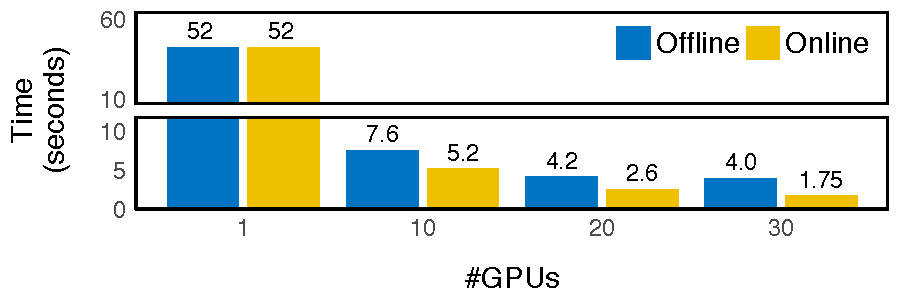
\includegraphics[width=0.8\columnwidth]{figures/parallel.pdf}
  \caption{Degradation-aware parallel scheduling}
  \label{fig:parallel}
\end{figure}

\para{Trigger-based profiling:} To avoid continuous profiling that requires
extensive CPU/GPU resources, our system only triggers profiling when it observed
significant difference between probe configurations and current
configurations. In our scheme, users can either configure the number of probe
configurations, or configure the available resources (CPU-time) and our system
will use offline profiles to calculate the corresponding trigger configurations.
\autoref{fig:online-tricks} shows how different numbers of trigger
configurations affects the profiling time. Notice that the continuous mode is
effectively probing all configurations (trigger($N$), $N$ is the total number of
all configurations).

Add subsample data (1 second duration vs. 5 seconds).

%%
%% Offline: 0
%% Online: 1 frame (1852.21 GPU * seconds)
%% Online (1/10)   (185.2 GPU * seconds)
%% Trigger         ( GPU * seconds)

\begin{figure}
  \centering
  \includegraphics[width=\columnwidth]{figures/online-profiling.pdf}
  \caption{Trigger-based profiling}
  \label{fig:online-tricks}
\end{figure}

\begin{table}
  \centering
  \begin{tabular}{c|c|c|c}
    \hline
    offline & online & online (partial) & online (trigger) \\
    \hline
    0       & 1852 (ms)   & 617 (ms)              & 223 (ms) \\
    \hline
  \end{tabular}
  \caption{Online Profiling Time}
  \label{tab:online}
\end{table}

\newpage

another column

\begin{figure*}[!htb]
  \begin{subfigure}[t]{0.3\textwidth}
    \centering
    \includegraphics[width=\textwidth]{figures/runtime-mot-verticle.pdf}
    \caption{Pedestrian Detection}
    \label{fig:pd-runtime}
  \end{subfigure}
  \hfill
  \begin{subfigure}[t]{0.3\textwidth}
    \centering
    \includegraphics[width=\textwidth]{figures/runtime-darknet-verticle.pdf}
    \caption{Augmented Reality}
    \label{fig:ar-runtime}
  \end{subfigure}
  \hfill
  \begin{subfigure}[t]{0.3\textwidth}
    \includegraphics[width=\textwidth]{figures/runtime-topk-verticle.pdf}
    \caption{Top-k}
    \label{fig:tk-runtime}
  \end{subfigure}
  \caption{Application profiles.}
  \label{fig:all-runtime}
\end{figure*}

\newpage

\subsection{Runtime Adaptation}
\label{sec:runtime-adaptation}

To evaluate the runtime behavior, we conduct controlled experiments using four
geo-distributed worker nodes from Amazon EC2 (t2.large instances) and an
aggregation server from our institute. For each experiment, worker nodes
transmit test data for about 10 mins. During each session, we use Linux
\texttt{tc} utility to adjust outgoing bandwidth to experiment with network
resource variation.

We show three aspects of the system: throughput, latency and application
accuracy. We compare our system with baseline systems that directly uses TCP and
UDP. In all three applications, the raw data streams are orders of magnitude
larger. While our system can adapt the rate, it could be unfair to baseline
solutions. We adjust the default degradation operation so that TCP and UDP would
work just fine when in normal cases; in this way, we make fair comparison. In
the case of UDP, shaping at the source doesn't emulate the packet loss behavior
with out-of-order delivery. We use \texttt{netem} to control packet loss rate to
match the desired shaping bandwidth.

From the throughput figure, we see how traffic shaping start, more severe
traffic shaping and traffic shaping stop affect the throughput. Notice that
after the traffic shaping stops, TCP has a ``catch-up'' phase where it's sending
all the queued items as fast as possible. Because of the queuing, TCP suffers
from an increased latency (as seen in the latency figure). But the data is
maintained at high fidelity in TCP, so the accuracy is always high. For UDP,
there is no explicit latency increase, but the accuracy drop is drastic during
traffic shaping.

Our run time adaptation achieves the balance between these two extremes: it has
low-latency (under 1 seconds) and high accuracy (above 85\%).

\newpage

another column

\newpage

\subsection{Multi-task Allocation}
\label{sec:multi-task-alloc}

At last the profile is useful for scheduling multiple stream processing
analytic. Applications doesn't behave well if they don't have the
adaptation. When their adaptation is turned on, but multiple tasks are
competing, some will suffer from the fair adaptation. This motivates us to
explore the multi-task scheduling.

There are mainly two schemes we are considering: (1) maximize the
\textit{minimum} utility (for \textit{MaxMin} fairness); (2) maximize the total
utility (for \textit{MaxTotal} performance). \autoref{fig:multitask} shows the
total utility of the baseline scheme and our two scheduling schemes.

\begin{figure}
  \centering
  \begin{subfigure}[t]{0.49\columnwidth}
    \centering
    \includegraphics[width=\textwidth]{figures/multitask-eq-bw.pdf}
    \caption{Equal Bandwidth}
    \label{fig:eq-bw}
  \end{subfigure}
  \hfill
  \begin{subfigure}[t]{0.49\columnwidth}
    \centering
    \includegraphics[width=\textwidth]{figures/multitask-eq-acc.pdf}
    \caption{Equal Acc}
    \label{fig:eq-acc}
  \end{subfigure}
  \caption{Multitask Allocation.}
  \label{fig:multitask}
\end{figure}

\newpage

%%% Local Variables:
%%% mode: latex
%%% TeX-master: "sosp17"
%%% End:
